\documentclass{if-beamer}

% --------------------------------------------------- %
%                  Presentation info	              %
% --------------------------------------------------- %
\title[Lecture 18]{Lecture 18}
\subtitle{Integration: Composite Trapezoid Rule, Recursion, and Simpson's 1/3 Rule}
\author{Ashley Gannon}
\date{ISC3313 Fall 2021}
\logo{

\includegraphics[scale=0.08]{figures/FSULogo.png}
}
\subject{Presentation subject}

% --------------------------------------------------- %
%                    Title + Schedule                 %
% --------------------------------------------------- %
\begin{document}

\begin{frame}
  \titlepage
\end{frame}
% --------------------------------------------------- %
%                      Presentation                   %
% --------------------------------------------------- %
\section{The Composite Trapezoid Rule Continued}

\begin{frame}
\frametitle{Let's think back to our formula}
If $a = x_0$ and $b=x_n$, the total integration with the trapezoidal rule can be represented by
$$I = h\frac{f(x_0)+f(x_1)}{2}+h\frac{f(x_1)+f(x_2)}{2}+...+h\frac{f(x_{n-1})+f(x_n)}{2}$$
If we expand this a bit more we can see a pattern emerge\\\vspace{5pt}
$I = h\frac{f(x_0)+f(x_1)}{2}+h\frac{f(x_1)+f(x_2)}{2}+h\frac{f(x_2)+f(x_3)}{2}+...+h\frac{f(x_{n-2})+f(x_{n-1})}{2}+h\frac{f(x_{n-1})+f(x_n)}{2}$\\\vspace{5pt}

And we can rewrite this equation as 
$$ I = \frac{h}{2}*(f(x_0)+f(x_n))+\frac{h}{2}\sum_{i=1}^{n-1}2f(x_i)$$ 
Which simplifies to
$$ I = \frac{h}{2}*(f(x_0)+f(x_n))+h\sum_{i=1}^{n-1}f(x_i)$$ 

\end{frame}

\begin{frame}
	\frametitle{The Composite Trapezoid Rule Pseudocode}
	
	\texttt{function takes in a, b, n}\\
	\texttt{declare/define h = (b-a)/n;}\\
	\texttt{declare/define sum = (h/2)*(f(a)+f(b)); }\\
	\texttt{declare/define xi = a+h;}\\
	\texttt{ }\\
	\texttt{loop over i = 1,...,n-1 }\\
	\texttt{\qquad add h*f(xi) to sum} \\
	\texttt{\qquad update xi = xi +h;}\\
	
\end{frame}	

\begin{frame}
	\frametitle{Thinking about the error}
	Last time we talked a bit about forming the error for the composite trapezoid rule.
	Recall that the error for the composite trapezoidal rule can be obtained by summing the individual errors for each segment to give
	$$ E_t = -\frac{(b-a)^3}{12n^3}\sum_{i+1}^{n}f''(\xi_i)$$
	Where $f''(x_i)$ is the second derivative at a point $\xi$ located in segment $i$. This result can be simplified by estimating the mean or average value of the second derivative for the entire interval as
	$$\bar{f}''\cong \frac{\sum_{i=1}^{n}f''(\xi_i)}{n} $$
	Subbing this into our equation for $E_t$, we can approximate the error $E_a$
	$$E_a = -\frac{(b-a)^3}{12n^2}\bar{f}''$$
	Where $\bar{f}''$ is found the same was as in the case of the single application of the trapezoidal rule. Which was done by finding the function's second derivative analytically,\\
	$f''(x) = -400+4050x-10800x^2+8000x^3$,
	to find $f''(\xi)$, and then taking the average value of the second derivative by computing
	$$ \bar{f}''(x) = \frac{\int_{0}^{0.8}(-400+4050x-10800x^2+8000x^3)dx}{0.8-0} = -60$$	
	
\end{frame}

\begin{frame}
	\frametitle{So how can we use this error to get a better result?}
	If we look at our function,
	$$E_a = -\frac{(b-a)^3}{12n^2}(-60) $$
	we notice that $E_a$ is only dependent on $n$ now that we have evaluated $\bar{f}''(x)$.  
	
\end{frame}

\begin{frame}
	\frametitle{So how can we use this error to get a better result?}
	If we look at our function,
	$$E_a = -\frac{(b-a)^3}{12n^2}(-60) $$
	we notice that $E_a$ is only dependent on $n$ now that we have evaluated $\bar{f}''(x)$. \\\vspace{10pt}
	If we want to modify our code so that this error falls below a desired tolerance, we will do this by using \textit{recursion}. 
	
\end{frame}

\begin{frame}[t]
	\frametitle{Recursion}
	\begin{itemize}
		\item In computer science, \textit{recursion} is a method of solving a problem where the solution depends on solutions to smaller instances of the same problem. \\\vspace{10pt}
	\end{itemize}
\end{frame}

\begin{frame}[t]
	\frametitle{Recursion}
	\begin{itemize}
		\item In computer science, \textit{recursion} is a method of solving a problem where the solution depends on solutions to smaller instances of the same problem. \\\vspace{10pt}
		\begin{itemize}
			\item So for this problem, we will take smaller and smaller segment sizes ($h$) until our error is less than our specified tolerance.$$-\frac{(b-a)^3}{12n^2}(-60) < tol $$\\\vspace{10pt}
		\end{itemize}
	\end{itemize}
\end{frame}

\begin{frame}[t]
	\frametitle{Recursion}
	\begin{itemize}
		\item In computer science, \textit{recursion} is a method of solving a problem where the solution depends on solutions to smaller instances of the same problem. \\\vspace{10pt}
		\begin{itemize}
			\item So for this problem, we will take smaller and smaller segment sizes ($h$) until our error is less than our specified tolerance.$$-\frac{(b-a)^3}{12n^2}(-60) < tol $$\\\vspace{10pt}
		\end{itemize}
		\item Recursive problems call themselves from within their own code. \\\vspace{10pt} 
	\end{itemize}
\end{frame}

\begin{frame}[t]
	\frametitle{Recursion}
	\begin{itemize}
		\item In computer science, \textit{recursion} is a method of solving a problem where the solution depends on solutions to smaller instances of the same problem. \\\vspace{10pt}
		\begin{itemize}
			\item So for this problem, we will take smaller and smaller segment sizes ($h$) until our error is less than our specified tolerance.$$-\frac{(b-a)^3}{12n^2}(-60) < tol $$\\\vspace{10pt}
		\end{itemize}
		\item Recursive problems call themselves from within their own code. \\\vspace{10pt} 
		\item The approach can be applied to many types of problems, and recursion is one of the central ideas of computer science.
	\end{itemize}
\end{frame}

\begin{frame}
	\frametitle{Recursive Composite Trapezoid Rule Pseudocode}
	\texttt{declare function that takes in a, b, n, $\bar{f}''$, tolerance}\\
	\texttt{ }
	\\\texttt{declare/define the error $-\frac{(b-a)^3}{12n^2}* \bar{f}''$}\\\vspace{2pt}
	\texttt{if error > tolerance}\\
	\texttt{This is where recursion comes in}\\
	\texttt{\qquad redefine n, n = 2*n for example}\\
	\texttt{\qquad return function(a,b,n,$\bar{f}''$, tol)}\\
	\texttt{ } \\
	\texttt{declare/define h = (b-a)/n;}\\
	\texttt{declare/define sum = (h/2)*(f(a)+f(b)); }\\
	\texttt{declare/define xi = a+h;}\\
	\texttt{ }\\
	\texttt{loop over i = 1,...,n-1 }\\
	\texttt{\qquad add h*f(xi) to sum} \\
	\texttt{\qquad update xi = xi +h;}\\
\end{frame}	

\section{Simpson's Rules}

\begin{frame}[t]
	\frametitle{Simpson's Rules}
	\begin{itemize}
		\item Aside from applying the trapezoidal rule with finer segmentation, another way to obtain
		a more accurate estimate of an integral is to use higher-order polynomials to connect the
		points
		
	\end{itemize}
\end{frame}	
	

\begin{frame}[t]
	\frametitle{Simpson's Rules}
	\begin{itemize}
		\item Aside from applying the trapezoidal rule with finer segmentation, another way to obtain a more accurate estimate of an integral is to use higher-order polynomials to connect the
		points
		\item For example, if there is an extra point midway between $f(a)$ and $f(b)$, the three
		points can be connected with a parabola
		\begin{figure}
			\centering
			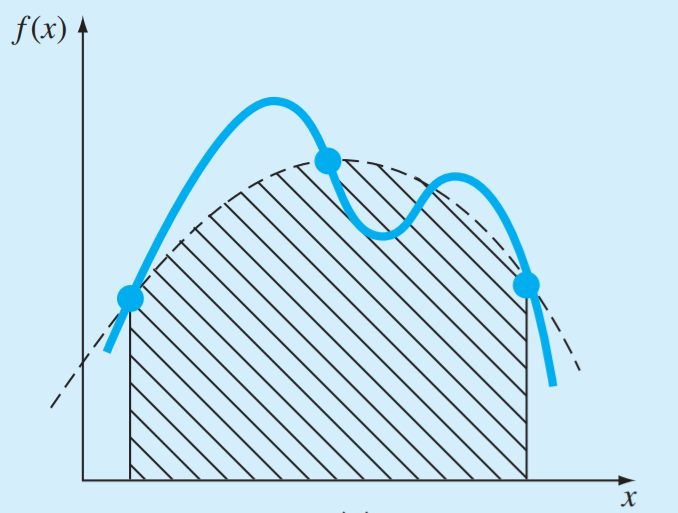
\includegraphics[width=0.25\textwidth]{figures/parab}
		\end{figure}
	\end{itemize}
\end{frame}	

\begin{frame}[t]
	\frametitle{Simpson's Rules}
	\begin{itemize}
		\item Aside from applying the trapezoidal rule with finer segmentation, another way to obtain a more accurate estimate of an integral is to use higher-order polynomials to connect the
		points
		\item For example, if there is an extra point midway between $f(a)$ and $f(b)$, the three
		points can be connected with a parabola
		\begin{figure}
			\centering
			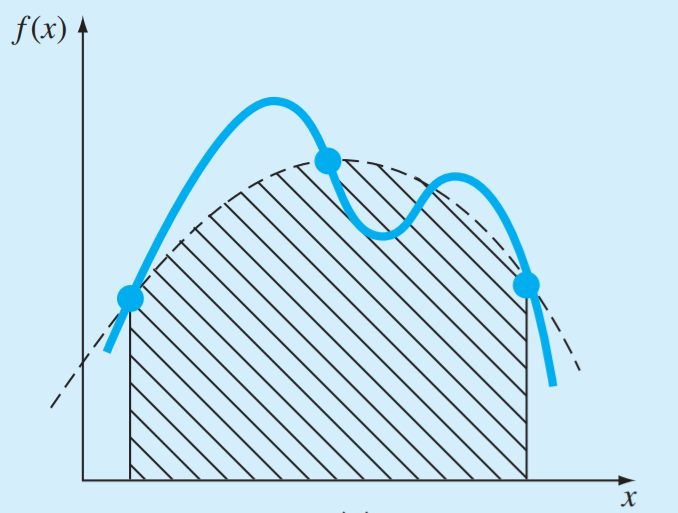
\includegraphics[width=0.25\textwidth]{figures/parab}
		\end{figure}
		\item  If there are two points equally spaced between $f(a)$ and $f(b)$, the four points can be connected with a third-order polynomial
		\begin{figure}
			\centering
			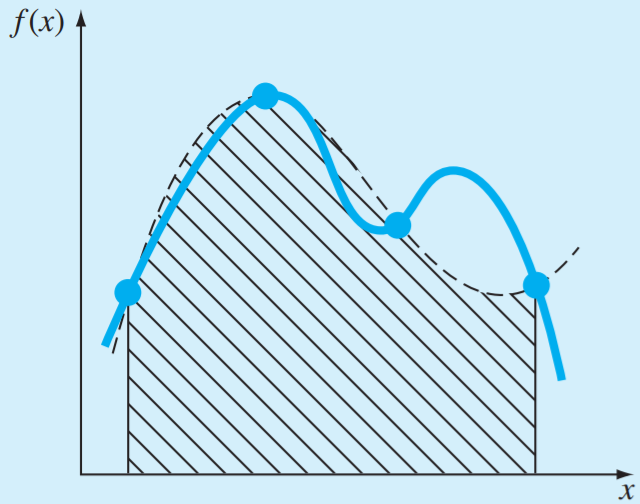
\includegraphics[width = 0.25\textwidth]{figures/other}
		\end{figure}
	\end{itemize}
\end{frame}	

\begin{frame}[t]
	\frametitle{Simpson's Rules}
	\begin{itemize}
		\item Aside from applying the trapezoidal rule with finer segmentation, another way to obtain a more accurate estimate of an integral is to use higher-order polynomials to connect the
		points
		\item For example, if there is an extra point midway between $f(a)$ and $f(b)$, the three
		points can be connected with a parabola
		\begin{figure}
			\centering
			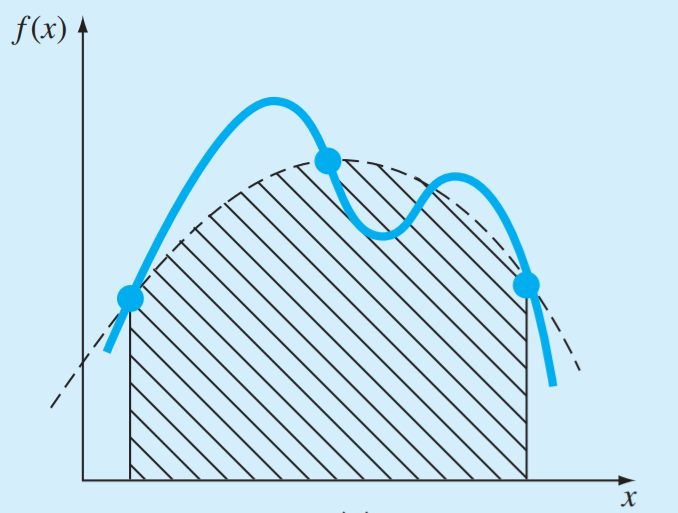
\includegraphics[width=0.25\textwidth]{figures/parab}
		\end{figure}
		\item  If there are two points equally spaced between $f(a)$ and $f(b)$, the four points can be connected with a third-order polynomial
		\begin{figure}
			\centering
			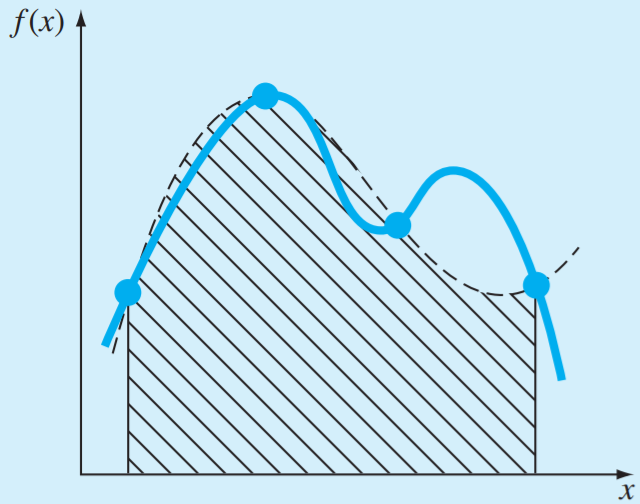
\includegraphics[width = 0.25\textwidth]{figures/other}
		\end{figure}
		\item  The formulas that result from taking the integrals under these
		polynomials are called \textit{Simpson’s rules.}
	\end{itemize}
\end{frame}	

\section{Simpson's 1/3 Rule}
\begin{frame}[t]
	\frametitle{Simpson's 1/3 Rule}
	Simpson's 1/3 rule corresponds to the case where the polynomial $f_n(x)$ in
	$$I \cong \int_{a}^{b}f_n(x)dx $$
	is 
	$$\frac{(x-x_1)(x-x_2)}{(x_0-x_1)(x_0-x_2)}f(x_0) + \frac{(x-x_0)(x-x_2)}{(x_1-x_0)(x_1-x_2)}f(x_1) + \frac{(x-x_0)(x-x_1)}{(x_2-x_0)(x_2-x_1)}f(x_2)$$

\end{frame}

\begin{frame}
	\frametitle{Simpson's 1/3 Rule}
	Simpson's 1/3 rule corresponds to the case where the polynomial $f_n(x)$ in
	$$I \cong \int_{a}^{b}f_n(x)dx $$
	is 
	$$\frac{(x-x_1)(x-x_2)}{(x_0-x_1)(x_0-x_2)}f(x_0) + \frac{(x-x_0)(x-x_2)}{(x_1-x_0)(x_1-x_2)}f(x_1) + \frac{(x-x_0)(x-x_1)}{(x_2-x_0)(x_2-x_1)}f(x_2)$$
	Plugging this in and integrating from $x_0$ to $x_2$
	\begin{align*}
		I &\cong \int_{x_0}^{x_2}\frac{(x-x_1)(x-x_2)}{(x_0-x_1)(x_0-x_2)}f(x_0) + \frac{(x-x_0)(x-x_2)}{(x_1-x_0)(x_1-x_2)}f(x_1) + \frac{(x-x_0)(x-x_1)}{(x_2-x_0)(x_2-x_1)}f(x_2)dx\\
	\end{align*}  
\end{frame}

\begin{frame}
	\frametitle{Simpson's 1/3 Rule}
	Simpson's 1/3 rule corresponds to the case where the polynomial $f_n(x)$ in
	$$I \cong \int_{a}^{b}f_n(x)dx $$
	is 
	$$\frac{(x-x_1)(x-x_2)}{(x_0-x_1)(x_0-x_2)}f(x_0) + \frac{(x-x_0)(x-x_2)}{(x_1-x_0)(x_1-x_2)}f(x_1) + \frac{(x-x_0)(x-x_1)}{(x_2-x_0)(x_2-x_1)}f(x_2)$$
	Plugging this in and integrating from $x_0$ to $x_2$
	\begin{align*}
		I &\cong \int_{x_0}^{x_2}\frac{(x-x_1)(x-x_2)}{(x_0-x_1)(x_0-x_2)}f(x_0) + \frac{(x-x_0)(x-x_2)}{(x_1-x_0)(x_1-x_2)}f(x_1) + \frac{(x-x_0)(x-x_1)}{(x_2-x_0)(x_2-x_1)}f(x_2)dx\\
		&=\frac{h}{3}(f(x_0)+4f(x_1)+f(x_2))\\
	\end{align*}  
\end{frame}
\begin{frame}
	\frametitle{Simpson's 1/3 Rule}
	Simpson's 1/3 rule corresponds to the case where the polynomial $f_n(x)$ in
	$$I \cong \int_{a}^{b}f_n(x)dx $$
	is 
	$$\frac{(x-x_1)(x-x_2)}{(x_0-x_1)(x_0-x_2)}f(x_0) + \frac{(x-x_0)(x-x_2)}{(x_1-x_0)(x_1-x_2)}f(x_1) + \frac{(x-x_0)(x-x_1)}{(x_2-x_0)(x_2-x_1)}f(x_2)$$
	Plugging this in and integrating from $x_0$ to $x_2$
	\begin{align*}
		I &\cong \int_{x_0}^{x_2}\frac{(x-x_1)(x-x_2)}{(x_0-x_1)(x_0-x_2)}f(x_0) + \frac{(x-x_0)(x-x_2)}{(x_1-x_0)(x_1-x_2)}f(x_1) + \frac{(x-x_0)(x-x_1)}{(x_2-x_0)(x_2-x_1)}f(x_2)dx\\
		&=\frac{h}{3}(f(x_0)+4F(x_1)+f(x_2))\\
	\end{align*}
	Where $x_0 = a$, $x_2 = b$ and $x_1$ is their midpoint, $x_1 = \frac{a+b}{2}$. This is known as \textit{Simpson's 1/3 Rule.} 
\end{frame}

\begin{frame}
	\frametitle{Error in Simpson's 1/3 Rule}
	It can be shown that a single-segment application of Simpson’s 1/3 rule has a truncation error of 
	$$E_t = -\frac{(b-a)^5}{2880}f^{(4)}(\xi)$$
	Where $\xi$ again lies somewhere on the interval from $a$ to $b$. We evaluate this term the same was as before by finding the average of the fourth derivative.
	$$ \bar{f}^{(4)} = \frac{\int_{a}^{b}f^{(4)}dx}{b-a}$$
\end{frame}

\begin{frame}
	\frametitle{Error in Simpson's 1/3 Rule}
	It can be shown that a single-segment application of Simpson’s 1/3 rule has a truncation error of 
	$$E_t = -\frac{(b-a)^5}{2880}f^{(4)}(\xi)$$
	Where $\xi$ again lies somewhere on the interval from $a$ to $b$.  We evaluate this term the same was as before by finding the average of the fourth derivative.
	$$ \bar{f}^{(4)} = \frac{\int_{a}^{b}f^{(4)}dx}{b-a}$$
	\begin{itemize}
		\item Simpson’s 1/3 rule is more accurate than the trapezoidal rule.
	\end{itemize}
\end{frame}

\begin{frame}
	\frametitle{Error in Simpson's 1/3 Rule}
	It can be shown that a single-segment application of Simpson’s 1/3 rule has a truncation error of 
	$$E_t = -\frac{(b-a)^5}{2880}f^{(4)}(\xi)$$
	Where $\xi$ again lies somewhere on the interval from $a$ to $b$. We evaluate this term the same was as before by finding the average of the fourth derivative.
	$$ \bar{f}^{(4)} = \frac{\int_{a}^{b}f^{(4)}dx}{b-a}$$
	\begin{itemize}
		\item Simpson’s 1/3 rule is more accurate than the trapezoidal rule.
		\item The Trapezoid rule error was proportional to the second derivative, Simpson's 1/3 rule is proportional to the fourth derivative
	\end{itemize}
\end{frame}

\begin{frame}
	\frametitle{Error in Simpson's 1/3 Rule}
	It can be shown that a single-segment application of Simpson’s 1/3 rule has a truncation error of 
	$$E_t = -\frac{(b-a)^5}{2880}f^{(4)}(\xi)$$
	Where $\xi$ again lies somewhere on the interval from $a$ to $b$. We evaluate this term the same was as before by finding the average of the fourth derivative.
	$$ \bar{f}^{(4)} = \frac{\int_{a}^{b}f^{(4)}dx}{b-a}$$
	\begin{itemize}
		\item Simpson’s 1/3 rule is more accurate than the trapezoidal rule.
		\item The Trapezoid rule error was proportional to the second derivative, Simpson's 1/3 rule is proportional to the fourth derivative
		\item Simpson's 1/3 rule is third order accurate and yields exact results for cubic polynomials even though it is derived from a parabola
	\end{itemize}
\end{frame}

\begin{frame}
	\frametitle{Single Application of Simpson’s 1/3 Rule}
	Let's use a single application of Simpson's 1/3 rule to numerically integrate
	$$f(x) =0.2+25x-200x^2+675x^3-900x^4+400x^5$$
	from $a = 0$ to $b=0.8$.
	Recalling our formula for Simpson's 1/3 rule is
	$$ I =\frac{h}{3}(f(x_0)+4f(x_1)+f(x_2))$$
\end{frame}

\begin{frame}
	\frametitle{Single Application of Simpson’s 1/3 Rule}
	Let's use a single application of Simpson's 1/3 rule to numerically integrate
	$$f(x) =0.2+25x-200x^2+675x^3-900x^4+400x^5$$
	from $a = 0$ to $b=0.8$.
	Recalling our formula for Simpson's 1/3 rule is
	$$ I =\frac{h}{3}(f(x_0)+4f(x_1)+f(x_2))$$
	The first thing we need to do is calculate the value for $x_1$
	$$x_1 = \frac{0.8+0}{2} = 0.4$$
\end{frame}

\begin{frame}
	\frametitle{Single Application of Simpson’s 1/3 Rule}
	Let's use a single application of Simpson's 1/3 rule to numerically integrate
	$$f(x) =0.2+25x-200x^2+675x^3-900x^4+400x^5$$
	from $a = 0$ to $b=0.8$.
	Recalling our formula for Simpson's 1/3 rule is
	$$ I =\frac{h}{3}(f(x_0)+4f(x_1)+f(x_2))$$
	The first thing we need to do is calculate the value for $x_1$
	$$x_1 = \frac{0.8+0}{2} = 0.4$$
	We can plug in the values for $h= \frac{0.8-0}{2}$, $f(0) = 0.2$, $f(0.4) =2.456$, and $f(0.8) = 0.232$
	$$ I = \frac{0.8-0}{2*3}(0.2+4(2.456)+0.232) = 1.367467$$
\end{frame}

\begin{frame}[t]
	\frametitle{Error in A Single Application of Simpson’s 1/3 Rule}
	Recalling our error formula
	$$E_t = -\frac{(b-a)^5}{2880}f^{(4)}(\xi)$$

\end{frame}

\begin{frame}[t]
	\frametitle{Error in A Single Application of Simpson’s 1/3 Rule}
	Recalling our error formula
	$$E_t = -\frac{(b-a)^5}{2880}f^{(4)}(\xi)$$
	We need to first evaluate $f^{(4)}(\xi)$ by finding the average of the fourth derivative.
	$$f^{(4)} = 48000x-21600$$
\end{frame}

\begin{frame}[t]
	\frametitle{Error in A Single Application of Simpson’s 1/3 Rule}
	Recalling our error formula
	$$E_t = -\frac{(b-a)^5}{2880}f^{(4)}(\xi)$$
	We need to first evaluate $f^{(4)}(\xi)$ by finding the average of the fourth derivative.
	$$f^{(4)} = 48000x-21600$$
	To find the average
	\begin{align*}
		\bar{f}^{(4)}(x) &= \frac{\int_{a}^{b}f^{(4)}(x)dx}{b-a}\\
		&= \frac{\int_{0}^{0.8}(48000x-21600)dx}{0.8-0}\\
		&= -2400\\
	\end{align*}
\end{frame}

\begin{frame}[t]
	\frametitle{Error in A Single Application of Simpson’s 1/3 Rule}
	Recalling our error formula
	$$E_t = -\frac{(b-a)^5}{2880}f^{(4)}(\xi)$$
	We need to first evaluate $f^{(4)}(\xi)$ by finding the average of the fourth derivative.
	$$f^{(4)} = 48000x-21600$$
	To find the average
	\begin{align*}
		\bar{f}^{(4)}(x) &= \frac{\int_{a}^{b}f^{(4)}(x)dx}{b-a}\\
		&= \frac{\int_{0}^{0.8}(48000x-21600)dx}{0.8-0}\\
		&= -2400\\
	\end{align*}
	Plugging this into our error we have
	$$E_a = -\frac{(0.8-0)^5}{2880}(-2400) = 0.2730667$$
\end{frame}

\begin{frame}[t]
	\frametitle{Composite Simpson's 1/3 Rule}
	Just as with the trapezoidal rule, Simpson’s rule can be improved by dividing the integration interval into a number of segments of equal width.
	\begin{figure}
		\centering 
		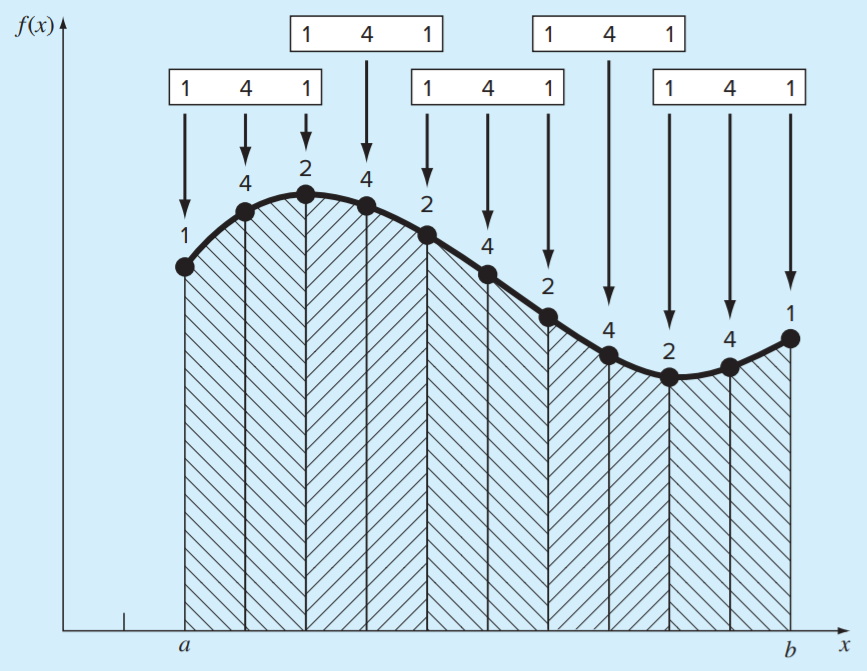
\includegraphics[width = 0.5\textwidth]{figures/compsimp}
	\end{figure}
    The total integration can be represented as
    $$ I = \int_{x_0}^{x_2}f(x)dx + \int_{x_2}^{x_4}f(x)dx + ... + \int_{x_{n-2}}^{x_n}f(x)dx$$
\end{frame}
\begin{frame}[t]
	\frametitle{Composite Simpson's 1/3 Rule}
	The total integration can be represented as
	$$ I = \int_{x_0}^{x_2}f(x)dx + \int_{x_2}^{x_4}f(x)dx + ... + \int_{x_{n-2}}^{x_n}f(x)dx$$

\end{frame}

\begin{frame}[t]
	\frametitle{Composite Simpson's 1/3 Rule}
	The total integration can be represented as
	$$ I = \int_{x_0}^{x_2}f(x)dx + \int_{x_2}^{x_4}f(x)dx + ... + \int_{x_{n-2}}^{x_n}f(x)dx$$
	Substituting Simpson’s 1/3 rule for each integral yields
	\begin{align*}
		I &= \frac{h}{3}(f(x_0)+4f(x_1)+f(x_2)) + \frac{h}{3}(f(x_2)+4f(x_3)+f(x_4))\\
		&+...+ \frac{h}{3}(f(x_{n-2})+4f(x_{n-1})+f(x_n))\\
	\end{align*}

\end{frame}

\begin{frame}[t]
	\frametitle{Composite Simpson's 1/3 Rule}
	The total integration can be represented as
	$$ I = \int_{x_0}^{x_2}f(x)dx + \int_{x_2}^{x_4}f(x)dx + ... + \int_{x_{n-2}}^{x_n}f(x)dx$$
	Substituting Simpson’s 1/3 rule for each integral yields
	\begin{align*}
		I &= \frac{h}{3}(f(x_0)+4f(x_1)+f(x_2)) + \frac{h}{3}(f(x_2)+4f(x_3)+f(x_4))\\
		&+...+ \frac{h}{3}(f(x_{n-2})+4f(x_{n-1})+f(x_n))\\
	\end{align*}
	Which can be re-written using summation notation
	$$I = \frac{h}{3}(f(x_0)+f(x_n))+\frac{h}{3}\left( 4\sum_{i = 1,3,5...}^{n-1}f(x_i) + 2\sum_{j = 2,4,6,...}^{n-2} f(x_j) \right)$$
\end{frame}

\begin{frame}[t]
	\frametitle{Composite Simpson's 1/3 Rule}
	The total integration can be represented as
	$$ I = \int_{x_0}^{x_2}f(x)dx + \int_{x_2}^{x_4}f(x)dx + ... + \int_{x_{n-2}}^{x_n}f(x)dx$$
	Substituting Simpson’s 1/3 rule for each integral yields
	\begin{align*}
		I &= \frac{h}{3}(f(x_0)+4f(x_1)+f(x_2)) + \frac{h}{3}(f(x_2)+4f(x_3)+f(x_4))\\
		&+...+ \frac{h}{3}(f(x_{n-2})+4f(x_{n-1})+f(x_n))\\
	\end{align*}
	Which can be re-written using summation notation
	$$I = \frac{h}{3}(f(x_0)+f(x_n))+\frac{h}{3}\left( 4\sum_{i = 1,3,5...}^{n-1}f(x_i) + 2\sum_{j = 2,4,6,...}^{n-2} f(x_j) \right)$$
	
	The coefficients 4 and 2 in might seem peculiar at first glance. However, they follow naturally from Simpson’s 1/3 rule, as
	illustrated in the previous/following image.
\end{frame}

\begin{frame}[t]
	\frametitle{Composite Simpson's 1/3 Rule}
	If we look back at the diagram for composite Simpson's 1/3 rule, 
	\begin{figure}
		\centering
		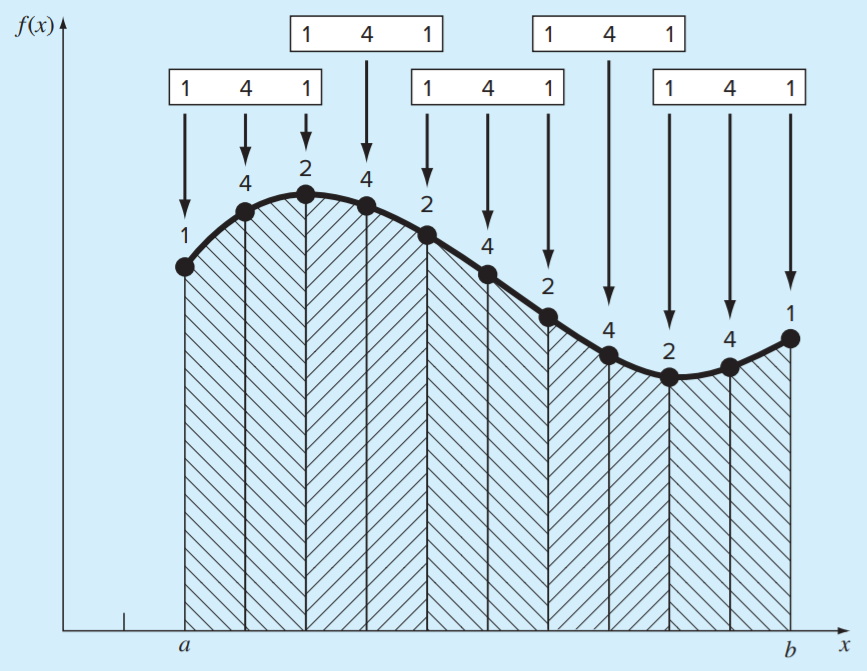
\includegraphics[width = 0.5\textwidth]{figures/compsimp}
	\end{figure}
	\begin{itemize}
		\item we notice that we must have an even number of segments to implement this method.\\
	\end{itemize} 
\end{frame}

\begin{frame}[t]
	\frametitle{Composite Simpson's 1/3 Rule}
	If we look back at the diagram for composite Simpson's 1/3 rule, 
	\begin{figure}
		\centering
		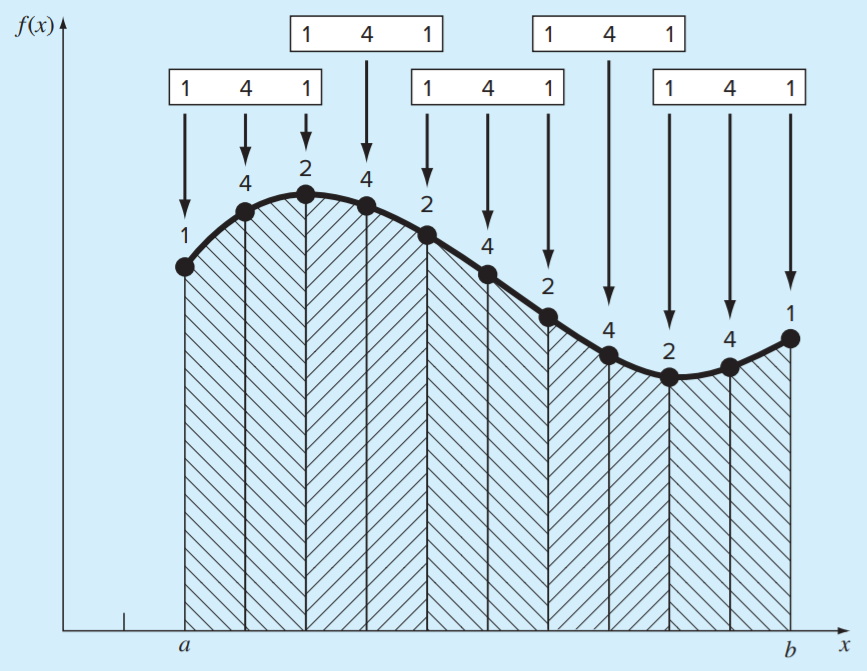
\includegraphics[width = 0.5\textwidth]{figures/compsimp}
	\end{figure}
	\begin{itemize}
		\item we notice that we must have an even number of segments to implement this method.\\
		\item We also can see from this figure that the odd points represent the middle term for each application which carry a weight of 4. \\
	\end{itemize} 
\end{frame}

\begin{frame}[t]
	\frametitle{Composite Simpson's 1/3 Rule}
	If we look back at the diagram for composite Simpson's 1/3 rule, 
	\begin{figure}
		\centering
		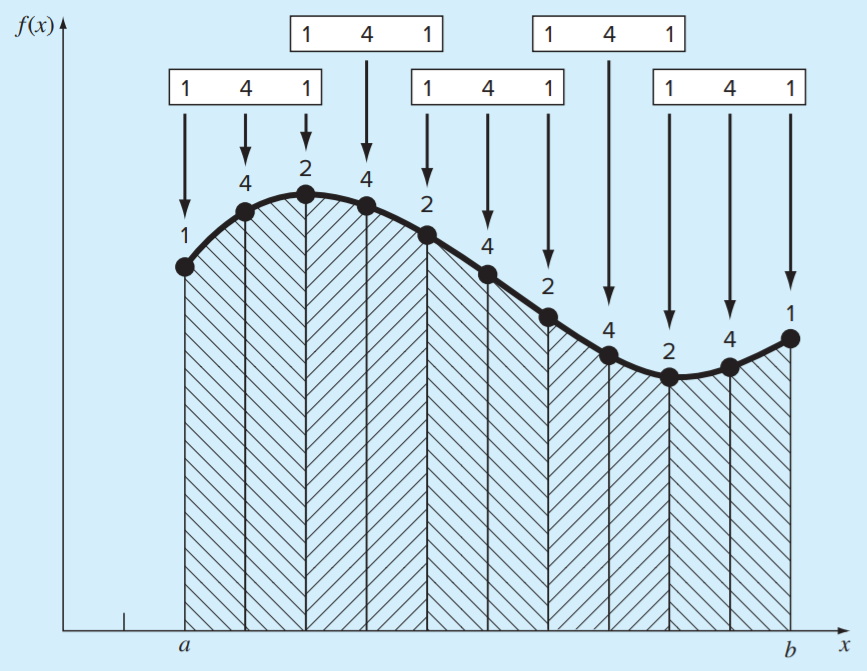
\includegraphics[width = 0.5\textwidth]{figures/compsimp}
	\end{figure}
	\begin{itemize}
		\item we notice that we must have an even number of segments to implement this method.\\
		\item We also can see from this figure that the odd points represent the middle term for each application which carry a weight of 4. \\
		\item And also that the even points are common to adjacent applications and are counted twice.
	\end{itemize} 
\end{frame}

\begin{frame}
	\frametitle{Error in Composite Simpson's 1/3 Rule}
	An error estimate for the composite Simpson’s rule is obtained in the same fashion as
	for the trapezoidal rule by summing the individual errors for the segments and averaging
	the derivative to yield
	$$ E_a = -\frac{(b-a)^5}{180n^4}\bar{f}^{(4)}$$
	where $f^{(4)}$ is the average fourth derivative for the interval.
\end{frame}

\begin{frame}[t]
	\frametitle{Composite Simpson’s 1/3 Rule Example}
	Let's use the composite Simpson's 1/3 rule to numerically integrate
	$$f(x) =0.2+25x-200x^2+675x^3-900x^4+400x^5$$
	from $a = 0$ to $b=0.8$, and $n =4$. \\\vspace{5pt}
	We first need to compute our $h$,
	$$h = \frac{0.8-0}{4} = 0.2$$

\end{frame}

\begin{frame}[t]
	\frametitle{Composite Simpson’s 1/3 Rule Example}
	Let's use the composite Simpson's 1/3 rule to numerically integrate
	$$f(x) =0.2+25x-200x^2+675x^3-900x^4+400x^5$$
	from $a = 0$ to $b=0.8$, and $n =4$. \\\vspace{5pt}
	We first need to compute our $h$,
	$$h = \frac{0.8-0}{4} = 0.2$$
	now we can compute our values for $x_1$, $x_2$, and $x_3$
	$$x_1 = a+h = 0.2$$
	$$x_2 = x_1 + h =0.4$$
	$$x_3 = x_2 +h = 0.6$$

\end{frame}

\begin{frame}[t]
	\frametitle{Composite Simpson’s 1/3 Rule Example}
	Let's use the composite Simpson's 1/3 rule to numerically integrate
	$$f(x) =0.2+25x-200x^2+675x^3-900x^4+400x^5$$
	from $a = 0$ to $b=0.8$, and $n =4$. \\\vspace{5pt}
	We first need to compute our $h$,
	$$h = \frac{0.8-0}{4} = 0.2$$
	now we can compute our values for $x_1$, $x_2$, and $x_3$
	$$x_1 = a+h = 0.2$$
	$$x_2 = x_1 + h =0.4$$
	$$x_3 = x_2 +h = 0.6$$
	And plug these values into $f$
	$$f(0) = 0.2$$
	$$f(0.2) = 1.288$$
	$$f(0.4) = 2.456$$
	$$f(0.6) = 3.464$$
	$$f(0.8) = 0.232$$
\end{frame}

\begin{frame}[t]
	\frametitle{Composite Simpson’s 1/3 Rule Example}
	Substituting these values into our equation
	$$I = \frac{h}{3}(f(x_0)+4f(x_1)+f(x_2)) + \frac{h}{3}(f(x_2)+4f(x_3)+f(x_4))$$
	We get
	$$I = \frac{0.8}{12}(0.2+4(0.2)+2(2.456)+2(3.464)+0.232) = 1.623467$$. 
\end{frame}

\begin{frame}[t]
	\frametitle{Composite Simpson’s 1/3 Rule Example}
	Substituting these values into our equation
	$$I = \frac{h}{3}(f(x_0)+4f(x_1)+f(x_2)) + \frac{h}{3}(f(x_2)+4f(x_3)+f(x_4))$$
	We get
	$$I = \frac{0.8}{12}(0.2+4(0.2)+2(2.456)+2(3.464)+0.232) = 1.623467$$
	Which has an approximate error of 
	$$E_a = -\frac{(b-a)^5}{180(4)^4}(-2400) = 0.017067$$
	which is 80\% less than the single application. 
\end{frame}


\begin{frame}
	\frametitle{Exercise}
	How would you code the composite Simpson's 1/3 rule? Write your pseudocode and submit it to the canvas discussion board \textbf{Composite Simpson's 1/3 Rule}. \\\vspace{10pt}
	
	NOTE: Use recursion to find the $n$ that drives the error to be less than your tolerance.
\end{frame}	
\end{document}
